\subsection{Kartoj}
%%%>>>>>>>>>>>>>>>>>>>>>>>>>>>>>>>>>>>>>>>>>>>>>>>>>>>>>>>>>>>>>>>>>>>>>>>>>>>>>>>>>>>>>>>>>>>>>>
  \begin{frame}
    \frametitle{Kion signifas vizaĝo sur karto?}
    \framesubtitle{Amrilato: ,,Tio estas komplika''}
	
	Eblas diversmaniere kompreni la fakton, ke iu estas ligita al la karto. Rekomendindas (laŭ PEJ spertoj) interkonsenti, ke estas kvar eblecoj:
	\begin{enumerate}
		\item vi \textbf{devas fari ion konkretan},
		\item vi \textbf{devas fari ion konkretan},
		\item vi \textbf{devas fari ion konkretan},
		\pause
		\item aŭ\dots \pause hispana inkvizicio \alert{(neniu atendis!)}.
	\end{enumerate}

  \end{frame}
%%%<<<<<<<<<<<<<<<<<<<<<<<<<<<<<<<<<<<<<<<<<<<<<<<<<<<<<<<<<<<<<<<<<<<<<<<<<<<<<<<<<<<<<<<<<<<<<<


%%%>>>>>>>>>>>>>>>>>>>>>>>>>>>>>>>>>>>>>>>>>>>>>>>>>>>>>>>>>>>>>>>>>>>>>>>>>>>>>>>>>>>>>>>>>>>>>>
  \begin{frame}
    \frametitle{Abonado de kartoj}
    \framesubtitle{Ja aboneblas ĝuste samkiel Kontakto!}
		
	Se vi bezonas nur esti informata, sed ankoraŭ ne havas konkretajn taskojn pri la temo ne aldonu sin al la karto -- \alert{ekzistas aliaj rimedoj por tio}:
	\begin{enumerate}
		\item abonu la karton (ekz. tre grava afero),
		\item abonu la tabulon (ekz. estrareca tabulo)
	\end{enumerate}
	
	\begin{columns}
    \column{0.3\textwidth}
	    \begin{block}{Karto}
	    	\begin{center}
	     	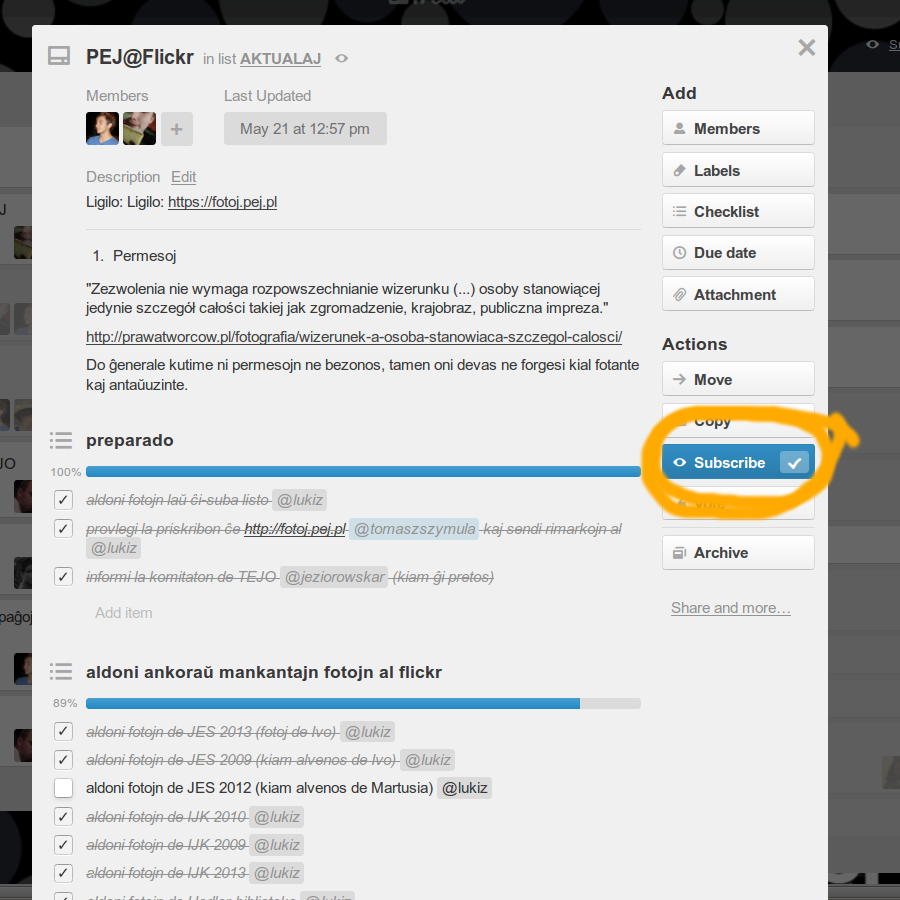
\includegraphics[scale=0.10]{ekranoj/abonu-karton}
	    	\end{center}
    	\end{block}
	\column{0.3\textwidth}
    	\begin{block}{Tabulo}
    		\begin{center}
    		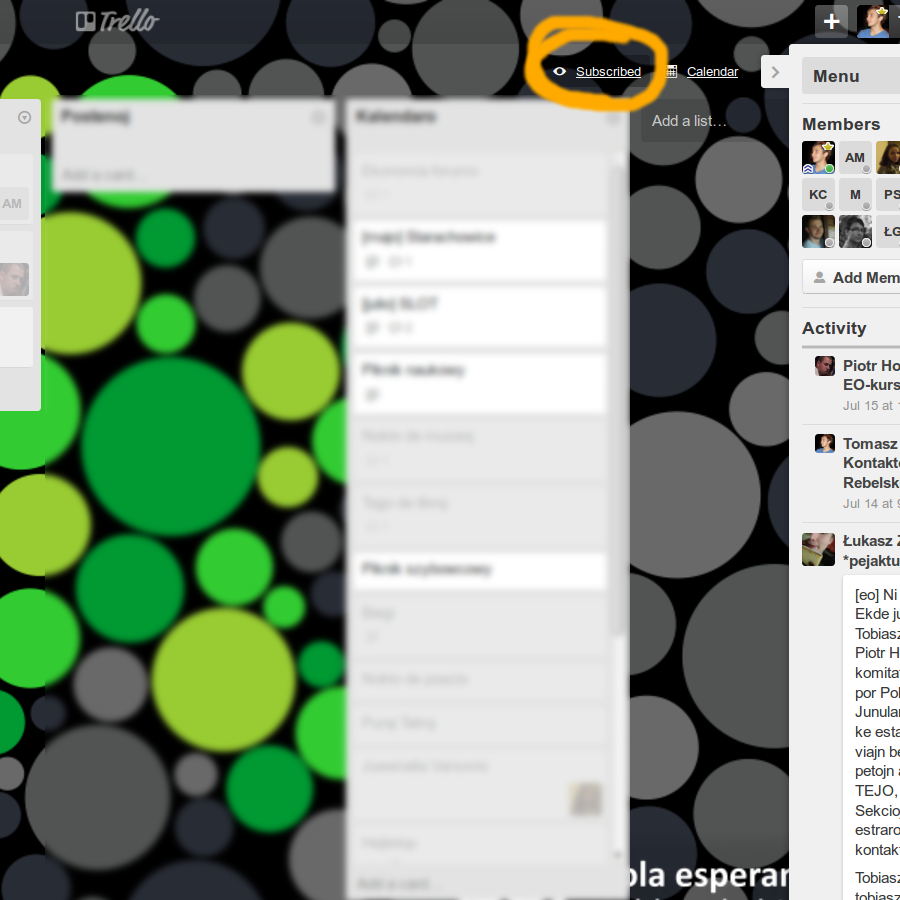
\includegraphics[scale=0.10]{ekranoj/abonu-tabulon}
    		\end{center}
    	\end{block}

	\end{columns}
  \end{frame}
%%%<<<<<<<<<<<<<<<<<<<<<<<<<<<<<<<<<<<<<<<<<<<<<<<<<<<<<<<<<<<<<<<<<<<<<<<<<<<<<<<<<<<<<<<<<<<<<<


%%%>>>>>>>>>>>>>>>>>>>>>>>>>>>>>>>>>>>>>>>>>>>>>>>>>>>>>>>>>>>>>>>>>>>>>>>>>>>>>>>>>>>>>>>>>>>>>>
  \begin{frame}
    \frametitle{Vi kaj la karto}
    \framesubtitle{Ĉu mi menciis tion?}
		
	Same, se vi volas nur informi iun (havigu al tiu persono la sciigon) malrekomendindas meti lin surkarten. Anstataŭ vi povas uzi "Menciu" funkcion.
\begin{center}

	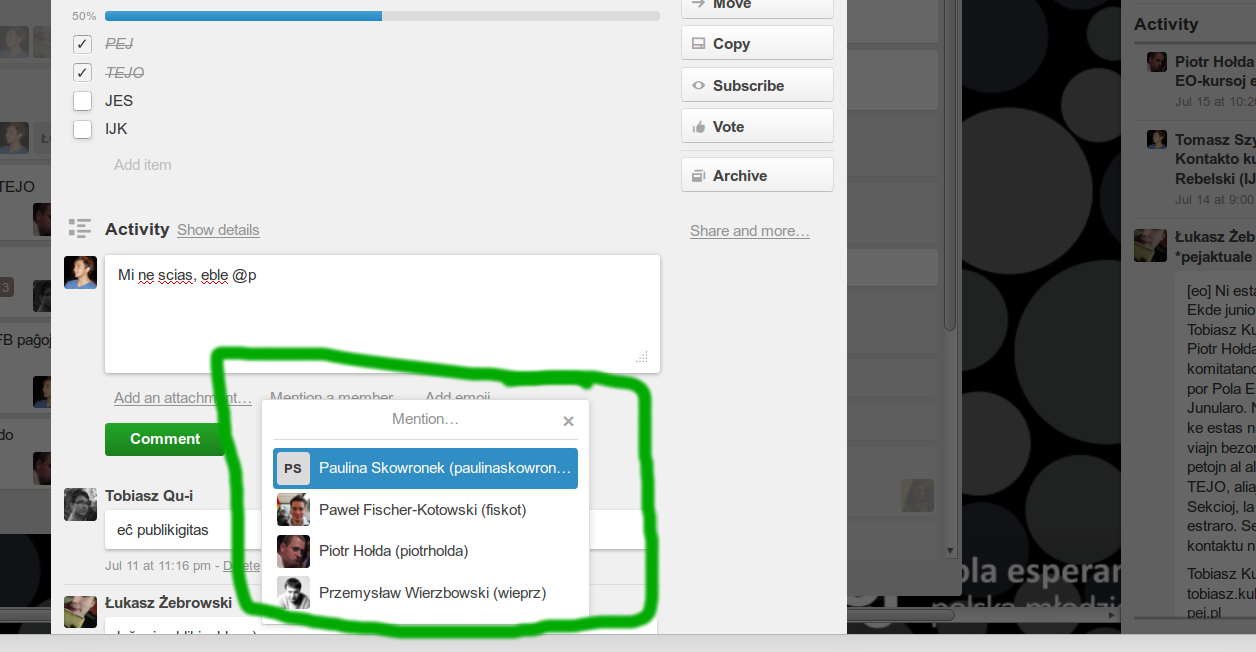
\includegraphics[scale=0.24]{ekranoj/mencio}

\end{center}
  \end{frame}
%%%<<<<<<<<<<<<<<<<<<<<<<<<<<<<<<<<<<<<<<<<<<<<<<<<<<<<<<<<<<<<<<<<<<<<<<<<<<<<<<<<<<<<<<<<<<<<<<

	    

%%%>>>>>>>>>>>>>>>>>>>>>>>>>>>>>>>>>>>>>>>>>>>>>>>>>>>>>>>>>>>>>>>>>>>>>>>>>>>>>>>>>>>>>>>>>>>>>>
  \begin{frame}
    \frametitle{Vi kaj la karto}
    \framesubtitle{Jam vi atendis, ĉu ne?}
	
	\begin{center}
		\begin{block}{Kontrola demando:}
			Kion signifas, se iu metis vin sur iu karto?
		\end{block}
	\end{center}
	
	\begin{center}
	    
\includegraphics[scale=0.3]{meme/hispana_inkvizicio}
    \end{center}	    
    
  \end{frame}
%%%<<<<<<<<<<<<<<<<<<<<<<<<<<<<<<<<<<<<<<<<<<<<<<<<<<<<<<<<<<<<<<<<<<<<<<<<<<<<<<<<<<<<<<<<<<<<<<
	    

%%%>>>>>>>>>>>>>>>>>>>>>>>>>>>>>>>>>>>>>>>>>>>>>>>>>>>>>>>>>>>>>>>>>>>>>>>>>>>>>>>>>>>>>>>>>>>>>>
  \begin{frame}
    \frametitle{Vi kaj la karto}
    \framesubtitle{Divenu laŭ jenaj informoj:}
    	
    \begin{columns}
    
    \column{0.5\textwidth}
    
    \begin{block}{Kiu reklamos?}
		
\includegraphics[scale=0.25]{ekranoj/kd-shangho}
    \end{block}
    
    \column{0.5\textwidth}
        
    \begin{block}{Kiu verkos?}    
    	
\includegraphics[scale=0.25]{ekranoj/artikolo-por-tt}
    \end{block}
    
    \end{columns}
  \end{frame}
%%%<<<<<<<<<<<<<<<<<<<<<<<<<<<<<<<<<<<<<<<<<<<<<<<<<<<<<<<<<<<<<<<<<<<<<<<<<<<<<<<<<<<<<<<<<<<<<<

%%%>>>>>>>>>>>>>>>>>>>>>>>>>>>>>>>>>>>>>>>>>>>>>>>>>>>>>>>>>>>>>>>>>>>>>>>>>>>>>>>>>>>>>>>>>>>>>>
  \begin{frame}
    \frametitle{Respondeco pri tasko}
    \framesubtitle{Kiel solvi?}

    \begin{columns}
    \column{0.6\textwidth}
    	
    ,,Tradicie'' marku en nomo de la karto. Funkcias tre bone.
    	
	\column{0.4\textwidth}
    
    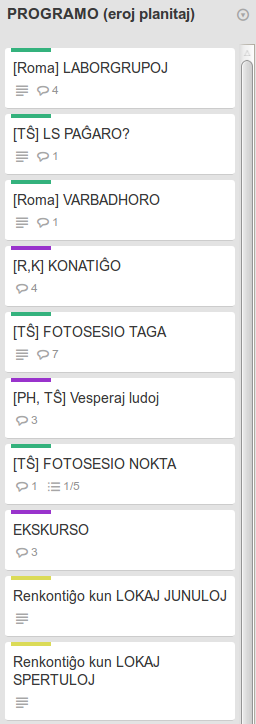
\includegraphics[scale=0.2]{ekranoj/respondeco-pri-karto}
	
	\end{columns}
  \end{frame}
%%%<<<<<<<<<<<<<<<<<<<<<<<<<<<<<<<<<<<<<<<<<<<<<<<<<<<<<<<<<<<<<<<<<<<<<<<<<<<<<<<<<<<<<<<<<<<<<<


%%%>>>>>>>>>>>>>>>>>>>>>>>>>>>>>>>>>>>>>>>>>>>>>>>>>>>>>>>>>>>>>>>>>>>>>>>>>>>>>>>>>>>>>>>>>>>>>>
  \begin{frame}
    \frametitle{Ĉiu projekto bezonas sian kunordiganton}

	\begin{block}{Praktika kaj efika difino}
		Kunordiganto de la projekto estas tiu, kiu devus honti, se la projekto malsukcesas. Pro tio liŝi zorgu, ke tio ne okazu.
	\end{block}
	    
  \end{frame}
%%%<<<<<<<<<<<<<<<<<<<<<<<<<<<<<<<<<<<<<<<<<<<<<<<<<<<<<<<<<<<<<<<<<<<<<<<<<<<<<<<<<<<<<<<<<<<<<<
